\documentclass{report}
\usepackage{amsmath, amssymb, amsthm}
\usepackage{physics}
\usepackage{float, subcaption, graphicx}
\usepackage{hyperref} % comment this in school template

\theoremstyle{plain}
\newtheorem{proposition}{Proposition}

\theoremstyle{definition}
\newtheorem{definition}{Definition}

\newtheorem{theorem}{Theorem}
\title{Instability In Magnetic Nozzle and Spectral Pollution}
\author{Hunt Feng}

% ABSTRACT


%%%%%%%%%%%%%%%%%%%%%%%%%%%%%%%%%%%%%%%%%%%%%%%%%%%%%%%%%%%%%%%%
% END OF FRONTMATTER SECTION
%%%%%%%%%%%%%%%%%%%%%%%%%%%%%%%%%%%%%%%%%%%%%%%%%%%%%%%%%%%%%%%%
\begin{document}
% Typeset the title page
\maketitle

\tableofcontents % remove this when using school template
% move abstract before the document in school template
\abstract{
    Spectral theory is a common technique for analyzing the instability of a dynamical system. By discretizing the linearized equations motion of magnetic nozzle, the instability problem becomes an algebraic eigenvalue problem. Given Dirichlet boundary condition, we found that the flow in magnetic nozzle is stable. Different discretizations, such as finite difference, finite element and DVR method agree with each other. By studying the convergence of different modes, we successfully eliminated the spurious unstable modes occur in supersonic and transonic cases. 
}

%%%%%%%%%%%%%%%%%%%%%%%%%%%%%%%%%%%%%%%%%%%%%%%%%%%%%%%%%%%%%%%%
% FIRST CHAPTER OF THESIS BEGINS HERE
%%%%%%%%%%%%%%%%%%%%%%%%%%%%%%%%%%%%%%%%%%%%%%%%%%%%%%%%%%%%%%%%
\chapter{Introduction}
\section{Motivation}
With the depletion of the earth's resources, the development of space has become a topic that cannot be avoided for mankind. To make space development possible, the necessary space propulsion technology must progress. 

To understand the advantage of electric propulsion. We need to review how propulsion system works. In order to change momentum, a spacecraft needs to expel parts of its mass, the propellant. The motion can be fully characterized by the Newton's second law.
\[ \dv{(mv_e)}{t} = \dot{m}v_e \]
where $m$ is the propellant mass, and $v_e$ is the exhaust velocity.

In 1903, a Russian and soviet rocket scientist, Konstantin Tsiolkovsky, derived the famous rocket equation that relates the change of a rocket's velocity to its exhaust velocity, and the mass of the rocket and propellant,
\[ \Delta v = -v_e \ln(\frac{M}{M+m}) \]
where $\delta v$ is the change in velocity of the spacecraft, $M$ is the mass of spacecraft without propellant, and $m$ is the mass of propellant.

From the Tsiolkovsky rocket equation, we see that higher the ratio between empty rocket and fueled rocket, higher the final velocity. Moreover, if the mass ratio is fixed, then a high exhaust velocity is needed in order to achieve higher final speed. In a chemical rocket, the exhaust velocity of propellant is limited by the temperature of the combustion fuels.

\begin{figure}[H]
	\centering
	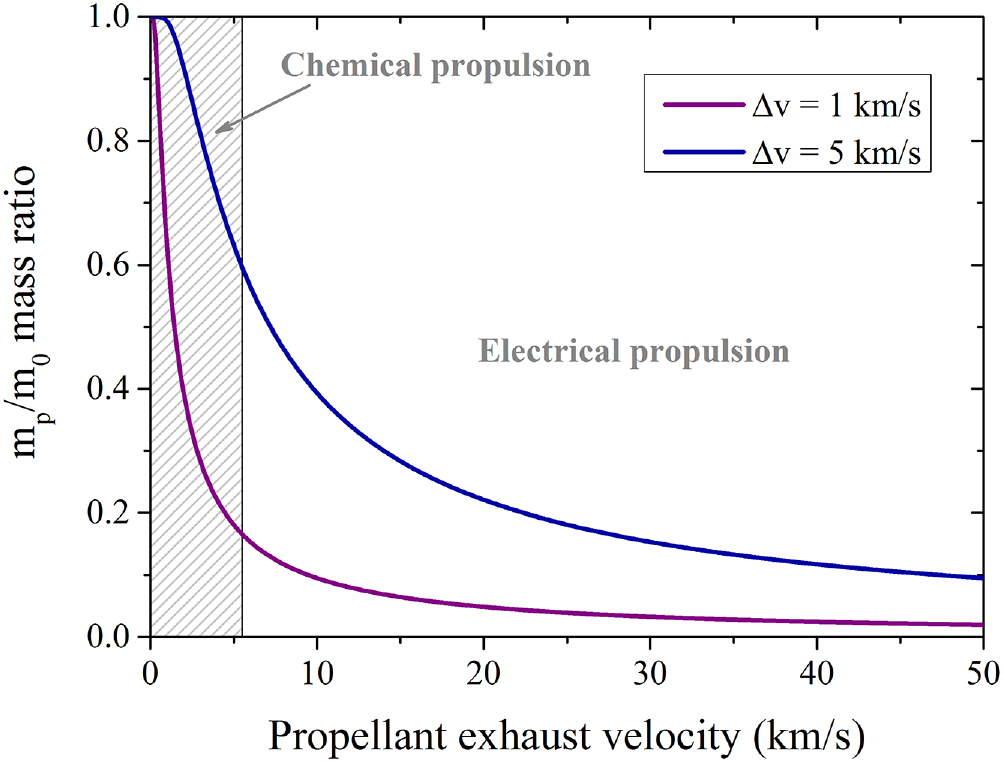
\includegraphics[width=0.7\linewidth]{img/introduction/mass_ratio_vs_exhaust_velocity}
	\caption{Ratio of the propellant mass to the initial mass as a function of the exhaust velocity ve for two values of the velocity increment $\Delta v$ . The dashed area corresponds to the domain of chemical propulsion with ve below 5.5 $km \, s^{-1}$. \cite{mazouffre_electric_2016} }
	\label{fig:massratiovsexhaustvelocity}
\end{figure}



\section{Magnetic Nozzle}
Magnetic nozzle is a convergent-divergent magnetic field that guides, expands and accelerates a plasma jet into vacuum for the purpose of space propulsion. \cite{andersen_continuous_1969,boswell_experimental_2004,williams_fusion_2003} The configuration is of the magnetic field in the magnetic nozzle plays a similar role to the walls of a Laval nozzle, see Fig. \ref{fig:magnetic-nozzle}. The plasma flow starts from subsonic at one end can be accelerated to supersonic at the other end. 

One advantage of magnetic nozzle is that it can operate contactlessly. Since the magnetic nozzle converts the plasma thermal energy into kinetic energy, so the thrust and specific impulse are strongly dependent on the temperature of the plasma flow. Higher the plasma temperature, more effective the plasma thruster. The magnetic field in the magnetic nozzle bounds the hot plasma, and therefore prevents the contact of the nozzle wall and the hot plasma jet. Hence, magnetic nozzle is an appealing plasma acceleration technology. Fig. \ref{fig:massratiovsexhaustvelocity} shows the comparison between magnetic nozzle and traditional chemical rocket.

Moreover, the configuration of magnetic field in magnetic nozzle is important for many other applications,\cite{smolyakov_quasineutral_2021} such as the magnetic divertors in fusion devices,\cite{ryutov_divertor_2016,togo_characteristics_2019} and is also related to the solar wind and accretion flow.\cite{jockers_stability_1968,aikawa_stability_1979} 

\begin{figure}[H]
	\centering
	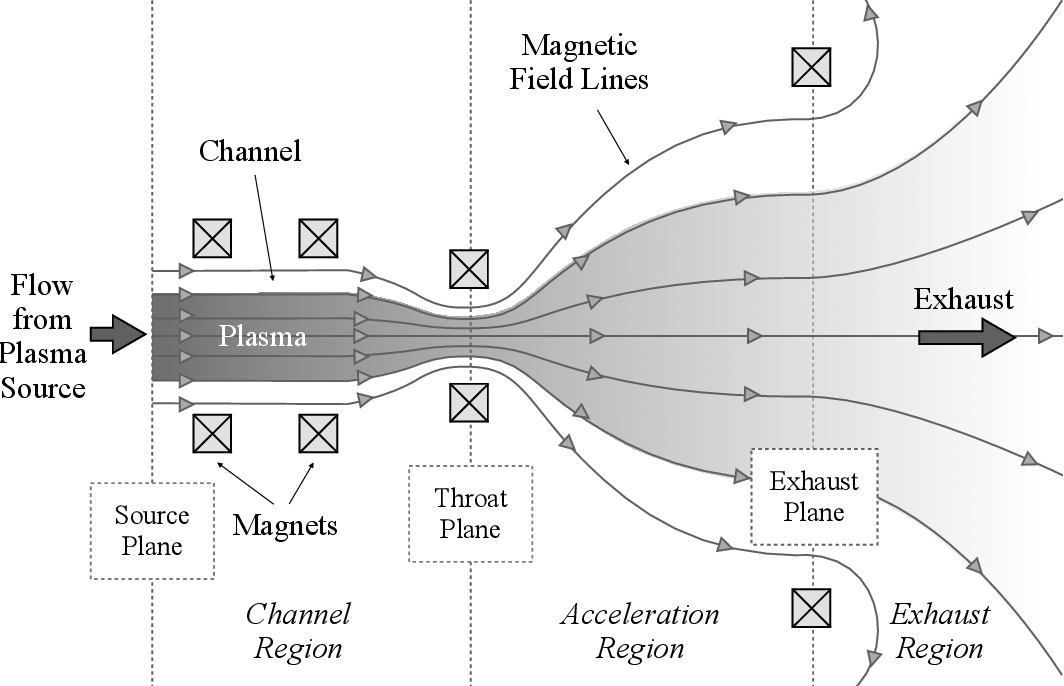
\includegraphics[width=0.7\linewidth]{img/introduction/magnetic_nozzle}
	\caption{Example of a magnetic nozzle configuration. In our models, we define the magnetic nozzle as the region downstream from the throat plane, which can be further divided into an acceleration region and exhaust region. The channel connects the plasma source (not shown) with the magnetic nozzle. \cite{little_performance_2015}}
	\label{fig:magnetic-nozzle}
\end{figure}


\section{Plasma Instability}
However, the plasma motion is determined by the Lorentz force, the nature of the nonlinearity of the motion makes it hard to predict analytically. Since the construction of Tokamak, people underestimated the difficulty of describing plasma motion. Hence, in order to maintain the equilibrium in the Tokamak, people start analyzing the stability of plasma. Nowadays, the study of plasma instabilities is an important area in plasma physics. 

Consider a plasma system in at equilibrium, we introduce a small perturbation to it. The stability of the system determines if the perturbations will grow, oscillate, or be damped out. Similar to the study of mechanical stability at equilibrium. See Fig. \ref{fig:stability-visualization}.

\begin{figure}[H]
	\centering
	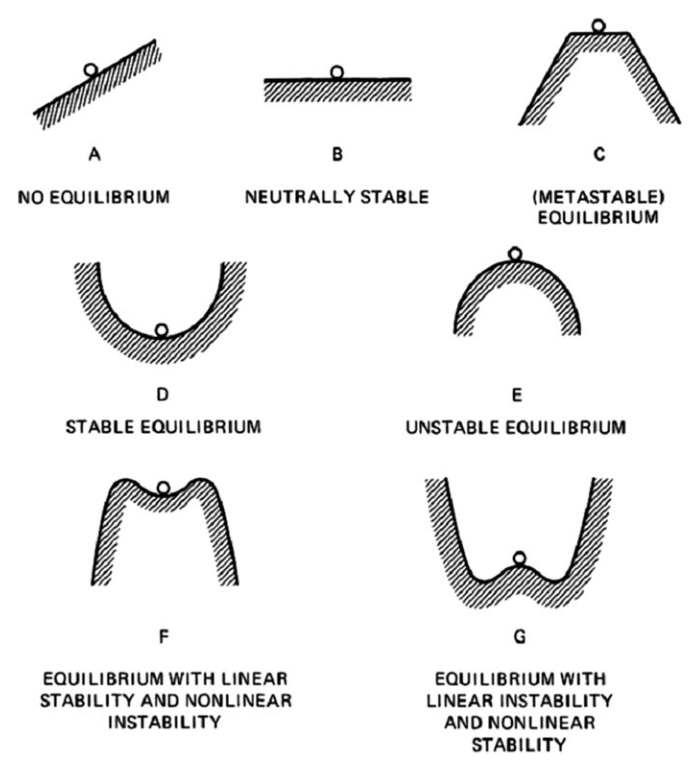
\includegraphics[width=0.7\linewidth]{img/introduction/stability_visualization}
	\caption{Mechanical analogy of various types of equilibrium. \cite{chen_introduction_2016}}
	\label{fig:stability-visualization}
\end{figure}


\subsection{Illustration: Two-Stream Instability}
We take the famous two-stream instability as an illustration. Let the plasma be cold ($k_BT_e = k_BT_i = 0$), let there be no magnetic field ($B_0=0$). The linearized continuity equations are
\begin{align} 
	\pdv{n_{i1}}{t} + n_0\pdv{v_{i1}}{x} &= 0  \label{eq:two-stream-continuity1} \\
	\pdv{n_{e1}}{t} + n_0\pdv{v_{e1}}{x} + v0\pdv{n_{e1}}{x} &= 0 \label{eq:two-stream-continuity2}
\end{align}

And the linearized equations of motion are
\begin{align} 
	Mn_0\pdv{v_{i1}}{t} &= en_0E_1  \label{eq:two-stream-eom1} \\
	mn_0\left(\pdv{v_{e1}}{t} + v_0\pdv{v_{e1}}{x}\right) &= -en_0E_1 \label{eq:two-stream-eom2}
\end{align}
Here $v_0$ is the velocity of electron respect to the ions (the ion velocity at equilibrium is taken to be $v_{i0}=0$), $n_0$ is the equilibrium density of both ion and electron, $v_{i1}$ and $v_{e1}$ are perturbed velocity of ions and electrons, and $E_1$ is the perturbed electron field.

If we assume perturbed electric field takes the wave form
\[ E_1 = E\exp(i(kx-\omega t)) \]
Plug this perturbed electric field into Eq.(\ref{eq:two-stream-eom1}) and (\ref{eq:two-stream-eom2}), then we can solve for $v_{i1}$ and $v_{e1}$,
\begin{align*}
	v_{i1} &= \frac{ie}{M\omega} E \\
	v_{e1} &= -\frac{ie}{m}\frac{E}{\omega-kv_0}
\end{align*}

Using the perturbed velocities, the continuity equations Eq.(\ref{eq:two-stream-continuity1}) and (\ref{eq:two-stream-continuity2}) yields
\begin{align*}
	n_{i1} &= \frac{ien_0k}{M\omega^2} E \\
	n_{e1} &= \frac{iekn_0}{m(\omega-kv_0)^2}E
\end{align*}

Finally, plug them into the Poisson's equation
\[ \epsilon_0 \pdv{E_1}{x} = e(n_{i1}-n_{e1}) \]
We now have the dispersion relation
\[ 1 = \omega_p \left[\frac{m/M}{\omega^2}+\frac{1}{(\omega-kv_0)^2}\right] \]

Solving this equation for $\omega$, there is chance we will get complex frequency,
\[ \omega = \omega_r + i\omega_i \]
where $\omega_r, \omega_i \in\mathbb{R}$. Then the perturbed electric field becomes
\[ E_1 = E\exp(i(kx-\omega_rt))\exp(\omega_it) \]

When $\omega_i < 0$, it is a damped wave, when $\omega_i > 0$, it grows exponentially and therefore unstable. Since the complex root comes with pair, as long as $\omega_i\neq 0$, one of the roots must correspond to an unstable wave. The following graph shows the two-stream instability in phase space.

\begin{figure}[H]
	\centering
	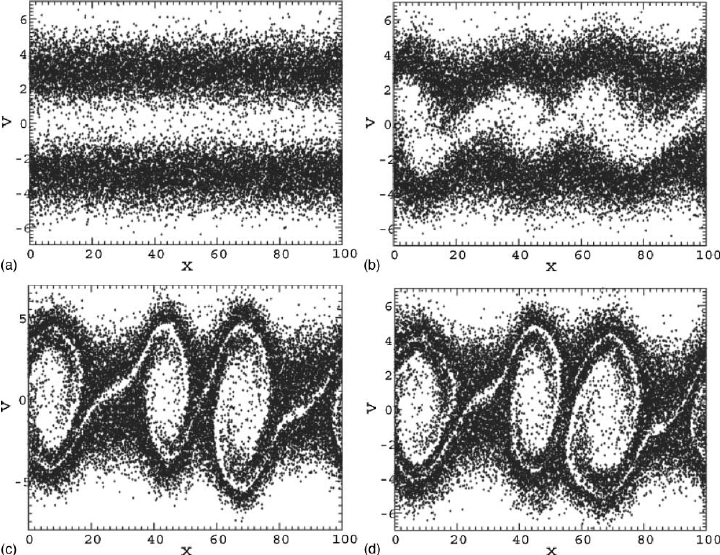
\includegraphics[width=0.7\linewidth]{img/introduction/two_stream_instability}
	\caption{Visualization of two-stream instability in the phase space. (a) Initially the ion and electron flow are in opposite direction. (b) The velocity of both flows start to oscillate. (c) Chaotic behavior occurs. (d) The chaotic behavior continues. \cite{ha_nonlinear_2011}}
	\label{fig:two_stream_instability}
\end{figure}

\subsection{Stability of Configurations Similar to Magnetic Nozzle}
Accretion flow has configuration similar to the magnetic nozzle. It is natural to find studies of stability the accretion flow. However, the results are still debatable. \cite{keto_stability_2020,aikawa_stability_1979,stellingwerf_stability_1978}


\section{Goals of this Thesis}
The goals of this thesis is to first study the spectral method for solving the instability problem. When using the spectral method, it is necessary to understand different discretizations of the operators, such as finite difference, finite element and DVR method.

Once the spectral method is introduced, we can use it to study the instability of plasma in magnetic nozzle. We can use different discretization techniques, and compare the results from different methods.

Finally, we need to take care of the filtering of the spectral pollution.


\section{Thesis Outline}
The theory of spectral methods will be discussed in chapter \ref{chap:spectral_method}. In this chapter, different discretiation methods will be introduced. Moreover, a very important concept, spectral pollution, will be introduced in detailed in the final section of this chapter.

Then, in chapter \ref{chap:governing_equations} is the discussion of governing equations and its linearization. The formulation of the problem will be derived in this chapter.

In chapter ??, we ill use the equations derived in chapter \ref{chap:governing_equations} to conduct numerical experiments. The goal is to investigate the frequency of each modes. The filtering methods of spurious modes will be introduced.

Conclusion will in chapter ??


\chapter{Spectral Method} \label{chap:spectral_method}
\section{Spectral Theory in Finite Dimensional Normed Spaces}
Let $X$ be a finite dimensional normed space and $\hat{T}: X \to X$ a linear operator. Since any linear operator can be represented by a matrix, the spectral theory of $\hat{T}$ is essentially matrix eigenvalue theory. \cite{kreyszig_introductory_1978} Let $A$ be a matrix representation of $\hat{T}$, then we have the definition.

\begin{definition}
	An eigenvalue of a square matrix $A$ is a complex number $\lambda$ such that
	\[ Ax = \lambda x \]
	has a solution $x\neq 0$.This $x$ is called an \textbf{eigenvector} of $A$ corresponding to that eigenvalue $\lambda$.The set $\sigma(A)$ of all eigenvalues of $A$ is called the \textbf{spectrum} of $A$. Its complement $\rho(A) = \mathbb{C}-\sigma(A)$ in the complex plane is called the \textbf{resolvent} set of $A$.
\end{definition}

By choosing different bases in $X$, we can have different matrix representation of $\hat{T}$. We need to make sure the eigenvalues of a linear operator is independent of the basis chosen. Fortunately, a theorem ensures that.

\begin{theorem}
	All matrices representing a given linear operator $\hat{T}: X \to X$ on a finite dimensional normed space $X$ relative to various bases for $X$ have the same eigenvalues.
\end{theorem}


Moreover, we don't need to worry about the existence of eigenvalues of a linear operator. The following theorem shows the existence of them.
\begin{theorem}
	A linear operator on a finite dimensional complex normed space $X\neq{O}$ has at least one eigenvalue.
\end{theorem}


\section{Spectral Theory in Normed Spaces of Any Dimension}
Let $X\neq {0}$ be a complex normed space (could be any dimension), and $\hat{T}: D(\hat{T}) \to X$ with domain $D(\hat{T}) \subset X$. Again, we could define eigenvalues, and other related concepts in terms of the equation
\[ \hat{T}x = \lambda x \]

\begin{definition}
	Let $\hat{T}\neq{0}$ be a complex normed space and $\hat{T}: D(\hat{T}) \to X$ a linear operator with domain $D(\hat{T})\subset X$. A \textbf{regular value} $\lambda$ of $\hat{T}$ is a complex number such that
	\begin{itemize}
		\item [(R1)] $(\hat{T}-\lambda I)^{-1}$ exists,
		\item [(R2)] $(\hat{T}-\lambda I)^{-1}$ is bounded,
		\item [(R3)] $(\hat{T}-\lambda I)^{-1}$ is defined on a set which is dense in $X$,
	\end{itemize}
	
	The \textbf{resolvent set} $\rho(\hat{T})$ of $\hat{T}$ is the set of all regular values $\lambda$ of $\hat{T}$. Its complement $\sigma(\hat{T}) = \mathbb{C} - \rho(\hat{T})$ in the complex plane $\mathbb{C}$ is called the \textbf{spectrum} of $\hat{T}$, and a $\lambda\in \sigma(\hat{T})$ is called a \textbf{spectral value} of $\hat{T}$. Furthermore, the spectrum $\sigma(\hat{T})$ is partitioned into three disjoint sets as follows.
	\begin{itemize}
		\item The \textbf{point spectrum} or \textbf{discrete spectrum} $\sigma_p(\hat{T})$ is the set such that $(\hat{T}-\lambda I)^{-1}$ does not exist. A $\lambda\in\sigma_p(\hat{T})$ is called an \textbf{eigenvalue} of $\hat{T}$.
		\item The \textbf{continuous spectrum} $\sigma_c(\hat{T})$ is the set such that $(\hat{T}-\lambda I)^{-1}$ exists and satisfies (R3) but not (R2), that is, $(\hat{T}-\lambda I)^{-1}$ is unbounded.
		\item The \textbf{residual spectrum} $\sigma_r(\hat{T})$ is the set such that $(\hat{T}-\lambda I)^{-1}$ exists (and may be bounded or not) but does not satisfy (R3), that is, the domain of $(\hat{T}-\lambda I)^{-1}$ is not dense in X.
	\end{itemize}
\end{definition}

In practice, the eigenvalue problem in infinite dimension is difficult. 
Therefore, the usual approach to the eigenvalue problem $\hat{T}x=\lambda x$ is to first discretize the operator $\hat{T}$ to an approximated matrix operator $T$, then the eigenvalue problem becomes,
\[ Tx = \lambda x \]

There are different ways to discretize the operator. For example, we can use finite difference, finite element and DVR methods. 

One important thing we need to keep in mind is that, the discretized version of the eigenvalue problem can have eigenvalues that are not in $\sigma(\hat{T})$. Those eigenvalues are called spurious eigenvalues, and this phenomenon is called spectral pollution. It is due to the improper discretization of the operators. We will discuss spectral pollution in the next section.

\section{Spectral Method}
Spectral method is one of the best tool to solve PDE and ODE problems. \cite{trefethen_spectral_nodate}. The central idea of spectral method is by discretizing the equation, we can transform that to a linear system or an eigenvalue problem.
\subsection{Finite Difference}
Consider equally spaced nodes on domain $[-1,1]$, $\{x_1, x_2, \dots, x_N\}$ with $x_{j+1}-x_{j} = h$ for each $j$, and the set of corresponding function values, $\{ f_1, f_2, \dots, f_N \}$. We can approximate the derivatives using second-order central difference formulas
\[ 
\pdv{f}{z} = \frac{f_{j+1} - f_{j-1}}{2h}
\qquad
\pdv[2]{f}{z} = \frac{f_{j+1} -2f_{j} +f_{j-1}}{h^2}
\]

We can discretize the differentiation operators to the following matrices
\[ 
\pdv{z} \rightarrow D = \frac{1}{2h}\begin{bmatrix}
	0 & 1 & 0 & \dots & 0 \\
	-1 & \ddots & \ddots & \ddots & \vdots \\ 
	0 & \ddots & \ddots & \ddots & 0 \\
	\vdots & \ddots & \ddots & \ddots & 1 \\
	0 & \dots & 0 & -1 & 0 
\end{bmatrix} 
\qquad
\pdv[2]{z} \rightarrow  D^2 = \frac{1}{h^2}\begin{bmatrix}
	-2 & 1 & 0 & \dots & 0 \\
	1 & \ddots & \ddots & \ddots & \vdots \\ 
	0 & \ddots & \ddots & \ddots & 0 \\
	\vdots & \ddots & \ddots & \ddots & 1 \\
	0 & \dots & 0 & 1 & -2 
\end{bmatrix} 
\]
\subsection{Finite Element}
Suppose the trial functions are $\{u_k(z)\}_{k=1}^\infty$, then the eigenfunction $\tilde{v}$ can be approximated by finite amount of them, $\tilde{v}(z) = \sum_{k=1}^N c_ku_k(z)$ where $c_k$ are coefficients to be determined.

Then by multiplying $u_{i}$ to any term and integrate through the domain, we can discretize the equation. Using the notation of inner product $(f,g)=\int_{-1}^{1} dz fg$, we see that

\[ \int_{-1}^{1} dz \; u_i\tilde{v} = \sum_{j}(u_i,u_j)c_j \]
\[ \int_{-1}^{1} dz \; u_i\pdv{\tilde{v}}{z} = \sum_{j}\left(u_i,\pdv{u_j}{z}\right)c_j \]
\[ \int_{-1}^{1} dz \; u_i\pdv[2]{\tilde{v}}{z} = \sum_{j}\left(u_i,\pdv[2]{u_j}{z}\right)c_j \]

\subsection{DVR Method}
\subsubsection{Sine DVR}
Let $\psi_n(z) = \sin(n\pi(z+1)/2)$, then we define $u_k$ using Gaussian quadrature, then
\[ u_k(z) = w_k\sum_{n=1}^N \psi_n(z)\psi_n^*(z_k) \]
where $w_k$ is the k-th weight for the Gaussian quadrature and $u_k$ satisfies the Kronecker delta property,
\[ u_j(x_k) = \delta_{jk} \]

Now the eigenfunction $\tilde{v} = \sum_{n=1}^N c_nu_n(z)$. The rest is the same as finite element, except the integrals are computed using Gaussian quadrature.

\subsubsection{Sinc DVR}
Let $sinc(x) = \sin(\pi x)/\pi x$, and define
\[ u_n(z) = \frac{1}{\sqrt{\Delta x}} sinc\left(\frac{x-x_q}{\Delta x}\right) \]
where $x_{q}$ are the quadrature points.
\chapter{Governing Equations} \label{chap:governing_equations}
\section{Single Particle Motion Along Magnetic Field Line}
The motion of charged particles in magnetic field is determined by the magnetic force,
\[ m\dv{\mathbf{v}}{t} = q\mathbf{v\times B} \]
where $m$ is the mass of charged particle, and $q$ is the charge of particles.

Consider a magnetic field pointing in z-direction, $\mathbf{B}=B\mathbf{\hat{z}}$. Since the magnetic force is perpendicular to both $\mathbf{v}$ and $\mathbf{B}$, we can separate the equation of motion into two directions,
\[ 
q\mathbf{v_{\perp}\times B} = \frac{mv_{\perp}^2}{r}\mathbf{\hat{r}}, 
\quad
\mathbf{v}_{\parallel} = v_{\parallel} \mathbf{\hat{z}} \]
where $\mathbf{v}_{\perp}$ is the velocity perpendicular to the magnetic field, and $\mathbf{v}_{\parallel}$ is the velocity parallel to the magnetic field. In this way, we see that the charged particle gyrates about the magnetic field, doing helical motion along the magnetic field line. 

Moreover, if we assume a static, nonuniform $\mathbf{B}$ field, the particles will stay on the same magnetic field line due to the so-called longitudinal invariant 
\[J = \int_{a}^{b} v_{\parallel} ds\]
where $[a,b]$ is the region of magnetic nozzle.  
\begin{figure}[H]
	\centering
	
\includegraphics[width=0.7\linewidth]{img/governing_equations/gyrate_along_b_field}
	\caption{A charged particle gyrates about the magnetic field line. The velocity along the field line is $\mathbf{v}_{\parallel}$ and the gyrate frequency, radius is given by the radial equation, $q\mathbf{v_{\perp}\times B} = \mathbf{\hat{r}} mv_\perp^2/r$. Moreover, for static, nonuniform magnetic field, the charged particle will stay on the same of magnetic field line as it gyrates.}
	\label{fig:gyrate-along-b-field}
\end{figure}


\section{From Kinetic Theory to Fluid Description}
In kinetic theory, the charged particles in plasma obey a certain distribution function $f(\mathbf{x}, \mathbf{v}, t)$. This distribution function is affected by plasma temperature. Assuming there is only one species of particles in the plasma, the plasma temperature is just the sum of the kinetic energy of all particles. We expect at higher temperature, faster the particles will be.

At equilibrium, the particles can be characterized by Maxwell-Boltzmann distribution
\[ f_M(\mathbf{x}, \mathbf{v}, t) = \frac{1}{(\pi v_{th}^2)^{3/2}} \exp(-\left(\frac{v}{v_{th}}\right)^2) \]
where $v_{th} = \sqrt{2k_BT/m}$ is the thermal velocity.

The moments of the distribution function are suitable macroscopic properties of the plasma. For example, the plasma density and plasma momentum can be viewed as 
\[ n(\mathbf{x}, t) = \int_{\mathbb{R}^3} f(\mathbf{x}, \mathbf{v}, t) d^3\mathbf{v} \]
\[ n\mathbf{V}(\mathbf{x}, t) = \int_{\mathbb{R}^3} \mathbf{v}f(\mathbf{x}, \mathbf{v}, t) d^3\mathbf{v} \]
where $\mathbf{V}$ is the fluid velocity of the charged particle. It is the bulk velocity of the plasma. In magnetic nozzle, since the charged particles flow along the magnetic field line, it is intuitive to think of $\mathbf{V}$ as the plasma flow velocity along the magnetic field line.

In fusion device and space propulsion system, we want high plasma temperature to achieve good performance. Hence, we assume high plasma temperature in this thesis. In other words, the plasma is collisionless. 

The distribution function $f$ in a collisionless plasma satisfies the so-called collisionless Vlasov equation, $\dv*{t} f(\mathbf{x}, \mathbf{v}, t) = 0$. Expand it explicitly, it is
\begin{equation} \label{eq:vlasov}
	\pdv{f}{t} + \mathbf{v}\pdv{f}{\mathbf{x}} + \frac{q}{m}(\mathbf{E} + \mathbf{v}\times\mathbf{B})\pdv{f}{\mathbf{v}} = 0
\end{equation}
where $q(\mathbf{E} + \mathbf{v}\times\mathbf{B})$ is the Lorentz force experience by the species, the collision term $C(f)$ is dropped. Worth to mention that the electric field and magnetic field are generated by the configuration and the motion of the charged particles.

Integrate both sides with respect to volume element in velocity space, $d^3\mathbf{v}$, we get the conservation of density.
\[ \pdv{\rho}{t} + \div(\rho\mathbf{V}) = 0 \]

If we multiply $\mathbf{v}$ on both sides and integrate with respect to $d^3\mathbf{v}$, we get the conservation of momentum.
\[ \rho\pdv{\mathbf{V}}{t} + \mathbf{V}\cdot\grad{\mathbf{V}} = \frac{q}{m}(\mathbf{E+V\times B}) - \grad{p} \]
In the process we assume isotropic pressure, and no viscosity exists in the plasma.

As we can see the fluid description only depends on the macroscopic properties of plasma, such as the fluid velocity along the magnetic field line $\mathbf{V}$, density $\rho$, and pressure $p$ of the plasma. This simplifies the problem.

\section{Governing Equations for Flow in Magnetic Nozzle}
In this section, we will derive the governing equations of the flow in magnetic nozzle, starting from the fluid description for plasma.

In magnetic nozzle, the magnetic field is along the nozzle, which we denote as z-axis. Due to Lorentz force, the charged particles gyrates about the magnetic field lines. Because the magnetic moment is invariant in such situation (\textbf{reference}). The fluid velocity of particles can be written as $\mathbf{v} = v\mathbf{B}/B$, meaning that the particles move along the magnetic field lines. Therefore the conservation of density 
\[ 
\pdv{n}{t} + \div(n\mathbf{v}) = 0 
\Rightarrow 
\pdv{n}{t} + B\pdv{z}(\frac{nv}{B}) = 0  
\]
In the derivation, $\div{\mathbf{B}} = 0$ is used.

To derive the second governing equation, we start from the conservation of momentum, 
\[ \pdv{v}{t} + v\pdv{v}{z} = -\frac{1}{\rho}\grad{p} \]
Let $\grad{p} = k_BT\pdv*{n}{z}$, we have
\[ \pdv{v}{t} + v\pdv{v}{z} = -c_s^2\frac{1}{n}\pdv{n}{z} \]
where $c_s^2 = k_BT/m$ is the square of sound speed.

Therefore the dynamics of the flow in magnetic nozzle can be characterized by the conservation of density and momentum,
\begin{align*}
	&\pdv{n}{t} + B\pdv{z}(\frac{nv}{B}) = 0\\
	&\pdv{v}{t} + v\pdv{v}{z} = -c_s^2\frac{1}{n}\pdv{n}{z}
\end{align*}
The discussion of magnetic field is in next subsection.


\subsection{Magnetic Field in Magnetic Nozzle}
In 1D problem, the magnetic field is given by
\[ B(z) = B_0 \left[1 + R\exp(-\left(\frac{x}{\delta}\right)^2)\right] \]
where $1+R$ is the magnetic mirror ratio, and $\delta$ determines the spread of the magnetic field. It is shown in Fig.(\ref{fig:magnetic-field}).
\begin{figure}[H]
	\centering
	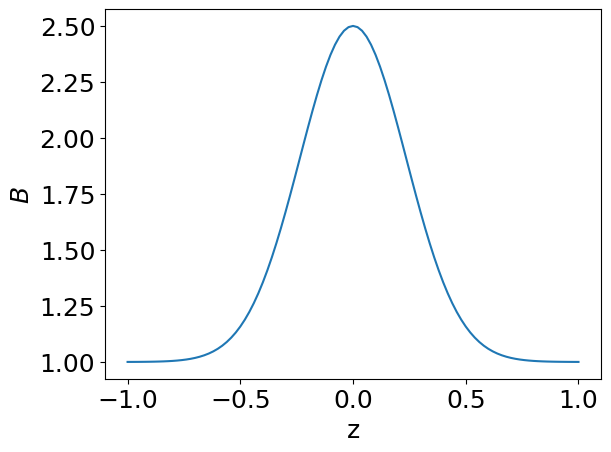
\includegraphics[width=0.7\linewidth]{img/governing_equations/magnetic_field}
	\caption{This is the magnetic field in nozzle with mirror ratio $1+R=B_{max}/B_{min}=2.5$, and the spread of magnetic field, $\delta=0.1/0.3=0.\bar{3}$. }
	\label{fig:magnetic-field}
\end{figure}


\subsection{Velocity Profile at Equilibrium}
Let $n_0$ and $v_0$ be the density and velocity at equilibrium (stationary solution), we know that $\pdv*{n_0}{t}=0$ and $\pdv*{v_0}{t}=0$, therefore $n_0$ and $v_0$ satisfy the so-called equilibrium condition,
\begin{align*}
	&\pdv{z}(\frac{n_0v_0}{B}) = 0 \\
	&v_0\pdv{v_0}{z} = -c_s^2\frac{1}{n_0}\pdv{n_0}{z} 
\end{align*}

Let $M(z) = v_0(z)/c_s$ be the mach number (nondimensionalized velocity). The equations of motion become
\begin{align*}
	&B\pdv{z}(\frac{n_0M}{B}) = 0\\
	&M\pdv{M}{z} = -\frac{1}{n_0}\pdv{n_0}{z}
\end{align*}
Substitute $\frac{1}{n_0}\pdv*{n_0}{z}$ using first equation, the conservation of momentum becomes
\[ (M^2-1)\pdv{M}{z} = -\frac{M}{B}\pdv{B}{z} \]

Notice that there is a singularity at $M=1$, the sonic speed.

This is a separable equation, integrate it and use the conditions at midpoint $B(0)=B_m, M(0)=M_m$ we get
\[ M^2e^{-M^2} = \frac{B^2}{B_m^2}M_m^2e^{-M_m^2} \]
We can now express $M$ using the Lambert W function,
\[ M(z) = \left[ -W_k\left(-\frac{B(z)^2}{B_m^2}M_m^2e^{-M_m^2}\right) \right]^{1/2} \]
where the subscript $k$ of $W$ stands for branch of Lambert W function. When $k=0$, it is the subsonic branch; When $k=-1$, it is the supersonic branch. Below shows a few cases of the solution.
\begin{itemize}
	\item $M_m < 1, k=0$, subsonic velocity profile.
	\item $M_m = 1$, $k=0$ for $x<0$ and $k=-1$ for $x>0$, accelerating profile
	\item $M_m = 1$, $k=-1$ for $x<0$ and $k=0$ for $x>0$, decelerating profile
	\item $M_m > 1, k=-1$, supersonic velocity profile
\end{itemize}
 Fig.(\ref{fig:velocity-profiles}) shows some cases of the solution.
\begin{figure}[H]
	\centering
	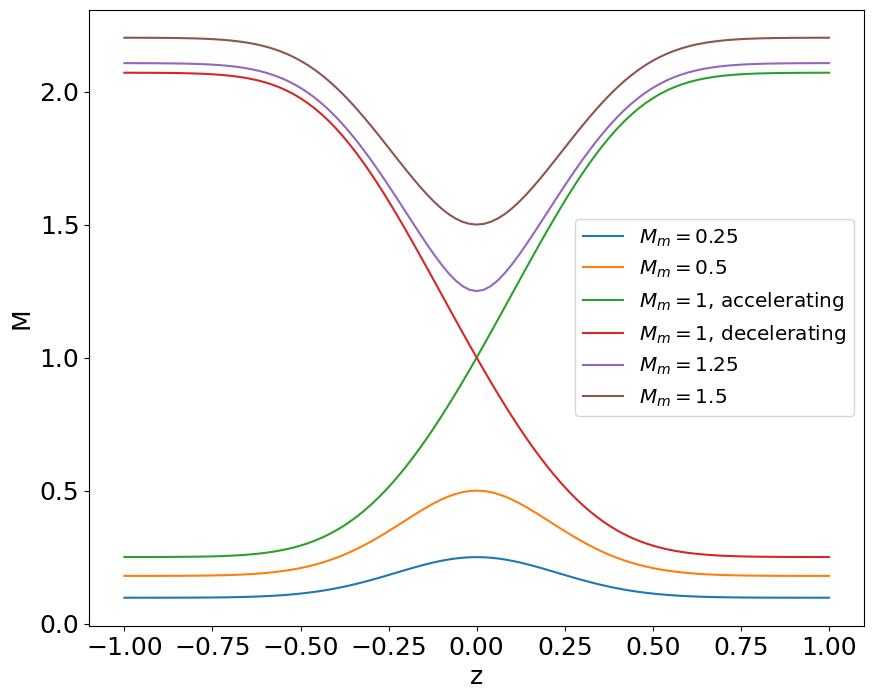
\includegraphics[width=0.7\linewidth]{img/governing_equations/velocity_profiles}
	\caption{The velocity profile in the magnetic nozzle is completely determined by $M_m$, the velocity at the midpoint, $z=0$. For the transonic velocity profiles, $M_m$ alone is not enough to determine the profile, we need to specify the branch of Lambert W function to determine whether it is accelerating or decelerating.}
	\label{fig:velocity-profiles}
\end{figure}



\section{Linearized Equations}
For convenience, we nondimensionalize the governing equations by normalizing the velocity to $c_s$, $v\mapsto v/c_s$, $z$ to system length $L$, $z \mapsto z/L$ and time $t\mapsto c_s t/L$. The governing equations become
\begin{align}
    &\pdv{n}{t} + n\pdv{v}{z} + v\pdv{n}{z} - nv\frac{\partial_z B}{B} = 0 \\
    &n\pdv{v}{t} + nv\pdv{v}{z} = -\pdv{n}{z}
\end{align}
and the nondimensionalized equilibrium condition is
\begin{align}
    &\pdv{z}(\frac{n_0v_0}{B}) = 0 \label{eq:equilibrium-convervation-of-mass}\\
    &v_0\pdv{v_0}{z} = -\frac{1}{n_0}\pdv{n_0}{z} \label{eq:equilibrium-convervation-of-momentum}
\end{align}

Now we are going to derive an important intermediate result, the linearized governing equations.
\begin{proposition}
    Let $n = n_0(z) + \tilde{n}(z,t)$ and $v = v_0(z) + \tilde{v}(z,t)$, where $\tilde{n}$ and $\tilde{v}$ are small perturbed quantities. The linearized governing equations are
    \begin{align}
        &\frac{1}{n_0}\pdv{\tilde{n}}{t} 
        + \pdv{\tilde{v}}{z} + v_0\tilde{Y} + \tilde{v}\frac{\partial_z n_0}{n_0} - \tilde{v}\frac{\partial_z B}{B} = 0 
        \label{eq:linearized-conservation-of-mass}
        \\
        &\pdv{\tilde{v}}{t} + \pdv{(v_0\tilde{v})}{z} = -\tilde{Y}
        \label{eq:linearized-conservation-of-momentum}
    \end{align}
    where 
    \[ \tilde{Y} \equiv \frac{1}{n_0}\pdv{\tilde{n}}{z} - \frac{\partial_z n_0}{n_0^2}\tilde{n} = \pdv{z}(\frac{\tilde{n}}{n_0}) \]
\end{proposition}
\begin{proof}
    We first derive Eq.(\ref{eq:linearized-conservation-of-mass}). We linearize Eq.(\ref{eq:equilibrium-convervation-of-mass}) by setting $n=n_0+\tilde{n}$ and $v=v_0+\tilde{v}$. By ignoring the second order perturbations, we obtain
    \begin{align*}
        &\pdv{(n_0+\tilde{n})}{t} 
        + (n_0+\tilde{n})\pdv{(v_0+\tilde{v})}{z} 
        + (v_0+\tilde{v})\pdv{(n_0+\tilde{n})}{z} 
        - (n_0+\tilde{n})(v_0+\tilde{v})\frac{\partial_z B}{B} = 0 \\
        \Rightarrow 
        &\pdv{\tilde{n}}{t} 
        + n_0\pdv{v_0}{z} + \tilde{n}\pdv{v_0}{z} + n_0\pdv{\tilde{v}}{z}
        + v_0\pdv{n_0}{z} + \tilde{v}\pdv{n_0}{z} + v_0\pdv{\tilde{n}}{z} 
        - (n_0v_0 + n_0\tilde{v} + \tilde{n}v_0)\frac{\partial_z B}{B} = 0 \\
        \Rightarrow
        &\frac{1}{n_0}\pdv{\tilde{n}}{t} 
        + \pdv{v_0}{z} + \frac{\tilde{n}}{n_0}\pdv{v_0}{z} + \pdv{\tilde{v}}{z}
        + \frac{v_0}{n_0}\pdv{n_0}{z} + \frac{\tilde{v}}{n_0}\pdv{n_0}{z} + \frac{v_0}{n_0}\pdv{\tilde{n}}{z} 
        - v_0\frac{\partial_z B}{B} - \tilde{v}\frac{\partial_z B}{B} - \tilde{n}\frac{v_0}{n_0}\frac{\partial_z B}{B} = 0
    \end{align*}
    Using the equilibrium condition Eq.(\ref{eq:equilibrium-convervation-of-mass}), some of the terms are canceled and the last term can be written as 
    \[ \tilde{n}\frac{v_0}{n_0}\frac{\partial_z B}{B} = \frac{\tilde{n}}{n_0}\left( \frac{\partial_z n_0}{n_0}v_0 + \pdv{v_0}{z} \right) \]
    Now, we are left with equation
    \[
        \frac{1}{n_0}\pdv{\tilde{n}}{t}
        + \pdv{\tilde{v}}{z}
        + v_0\underbrace{\left(\frac{1}{n_0}\pdv{\tilde{n}}{z} - \frac{\tilde{n}}{n_0}\frac{\partial_z n_0}{n_0}  \right)}_{\tilde{Y}}
        + \frac{\tilde{v}}{n_0}\pdv{n_0}{z}
        - \tilde{v}\frac{\partial_z B}{B} = 0
    \]

    To derive Eq.(\ref{eq:linearized-conservation-of-momentum}), we linearize the LHS of the conservation of momemtum
    \begin{align*}
        &(n_0+\tilde{n})\pdv{(v_0+\tilde{v})}{t} + (n_0+\tilde{n})(v_0+\tilde{v})\pdv{(v_0+\tilde{v})}{z} = -\pdv{n}{z} \\
        \Rightarrow 
        & \pdv{v_0}{t} + \frac{\tilde{n}}{n_0}\pdv{v_0}{t} + \pdv{\tilde{v}}{t} 
        + \left(v_0+\tilde{v}+\frac{\tilde{n}}{n_0}v_0\right)\pdv{(v_0+\tilde{v})}{z} = -\frac{1}{n_0}\pdv{n}{z}\\
        \Rightarrow
        & \pdv{v_0}{t} + v_0\pdv{v_0}{z} + \tilde{v}\pdv{v_0}{z} 
        = -\frac{1}{n_0}\pdv{n_0}{z} -\frac{1}{n_0}\pdv{\tilde{n}}{z} -v_0\frac{v_0}{z} - \frac{\tilde{n}}{n_0}v_0\pdv{v_0}{z} \\ 
    \end{align*}
    Using the equilibrium condition Eq.(\ref{eq:equilibrium-convervation-of-momentum}) on the RHS, we get the desired form.
\end{proof}


\section{Formulation of the Problem}
In order to investigate the instability of magnetic nozzle, we need formulate it as an eigenvalue problem. To do that, we assume the perturbed density and velocity are oscillatory, i.e. $\tilde{n}, \tilde{v} \sim \exp(-i\omega t)$, where $\omega$ is the oscillation frequency of the perturbed quantities. This frequency can be a complex number. If $\omega = \omega_r +i \omega_i$, then the perturbed quantities becomes $\tilde{n} \sim \exp(\omega_i t)\exp(i\omega_r t)$, which means it grows exponentially with time.

The first step, we can combine Eq.(\ref{eq:linearized-conservation-of-mass}) and Eq.(\ref{eq:linearized-conservation-of-momentum}) into 1 equation.
\begin{proposition}
	\begin{equation}
		\pdv{z}\ln(\frac{n_0}{B}) = -\frac{1}{v_0}\pdv{v_0}{z}
		\label{eq:dv-ln}
	\end{equation}
\end{proposition}
\begin{proof}
	\[ \pdv{z}\ln(\frac{n_0}{B}) 
	= \frac{B}{n_0}\pdv{z}(\frac{n_0}{B})
	= \frac{1}{n_0}\frac{n_0}{z} + B\pdv{z}(\frac{1}{B})
	=
	\frac{1}{n_0}\frac{n_0}{z} \underbrace{- \frac{1}{n_0v_0}\pdv{n_0v_0}{z}}_{Eq.(\ref{eq:equilibrium-convervation-of-mass})}
	= -\frac{1}{v_0}\pdv{v_0}{z} \]
\end{proof}

\begin{proposition}
	Let $\tilde{n}\sim \exp(-i\omega t)$ and $\tilde{v} \sim \exp(-i\omega t)$, then we have the polynomial eigenvalue problem
	\begin{equation}
		\hspace{-0.5in}
		\omega^2 \tilde{v} 
		+ 2i\omega\left(v_0\pdv{}{z} + \pdv{v_0}{z}\right) \tilde{v} 
		+ \left[ (1-v_0^2)\pdv[2]{}{z} 
		-\left(3v_0 + \frac{1}{v_0}\right)\pdv{v_0}{z}\pdv{}{z} 
		- \left(1-\frac{1}{v_0^2}\right)\left(\pdv{v_0}{z}\right)^2 
		- \left(v_0+\frac{1}{v_0}\right)\pdv[2]{v_0}{z} \right]\tilde{v}
		= 0
		\label{eq:polynomial-eigenvalue-problem}
	\end{equation}
\end{proposition}
\begin{proof}
	\begin{align*}
		&\frac{1}{n_0}\pdv{\tilde{n}}{t} 
		+ \pdv{\tilde{v}}{z} + v_0\tilde{Y} + \tilde{v}\frac{\partial_z n_0}{n_0} - \tilde{v}\frac{\partial_z B}{B} = 0 
		\\
		&\pdv{\tilde{v}}{t} + \pdv{(v_0\tilde{v})}{z} = -\tilde{Y}
	\end{align*}
	
	
	We plug Eq.(\ref{eq:linearized-conservation-of-momentum}) in to Eq.(\ref{eq:linearized-conservation-of-mass}), we have 
	\[ -i\omega\frac{\tilde{n}}{n_0} 
	+ \pdv{\tilde{v}}{z} - v_0\left(-i\omega\tilde{v} + \pdv{(v_0\tilde{v})}{z}\right) + \tilde{v}\frac{\partial_z n_0}{n_0} - \tilde{v}\frac{\partial_z B}{B} = 0 \]
	
	Using the equilibrium condition Eq.(\ref{eq:equilibrium-convervation-of-mass}), we can eliminate the term $\partial_z B/B$,
	\begin{align*}
		&-i\omega\frac{\tilde{n}}{n_0} 
		+ \pdv{\tilde{v}}{z} 
		+ v_0\left(i\omega \tilde{v} - v_0\pdv{\tilde{v}}{z} - \tilde{v}\pdv{v_0}{z} \right)
		- \tilde{v}\frac{\partial_z v_0}{v_0} = 0\\
		\Rightarrow
		&-i\omega\frac{\tilde{n}}{n_0} 
		+ i\omega v_0\tilde{v}
		+ (1-v_0^2)\pdv{\tilde{v}}{z} 
		- \left(v_0+\frac{1}{v_0}\right)\pdv{v_0}{z}\tilde{v} = 0
	\end{align*}
	
	Now we take $\pdv*{t}$ on Eq.(\ref{eq:linearized-conservation-of-momentum}). Recall the fact that $\tilde{Y} = \pdv*{(\tilde{n}/n_0)}{z}$, we have
	\begin{align*}
		\omega^2\tilde{v} + i\omega\left(v_0\pdv{\tilde{v}}{z} + \tilde{v}\pdv{v_0}{z}\right) &= \pdv{t}\pdv{z}(\frac{\tilde{n}}{n_0}) \\
		\Rightarrow
		\omega^2\tilde{v} + i\omega\left(v_0\pdv{\tilde{v}}{z} + \tilde{v}\pdv{v_0}{z}\right) &= \pdv{z}(-i\omega v_0\tilde{v}
		- (1-v_0^2)\pdv{\tilde{v}}{z} 
		+ \left(v_0+\frac{1}{v_0}\right)\pdv{v_0}{z}\tilde{v})
	\end{align*}
	Expand the RHS and collect terms, we get
	\begin{align*}
		&\omega^2 \tilde{v} \\ 
		&+2i\omega\left(v_0\pdv{}{z} + \pdv{v_0}{z}\right) \tilde{v} \\ 
		&+\left[ (1-v_0^2)\pdv[2]{}{z} 
		-\left(3v_0 + \frac{1}{v_0}\right)\pdv{v_0}{z}\pdv{}{z} 
		- \left(1-\frac{1}{v_0^2}\right)\left(\pdv{v_0}{z}\right)^2 
		- \left(v_0+\frac{1}{v_0}\right)\pdv[2]{v_0}{z} \right]\tilde{v}
		= 0
	\end{align*}
\end{proof}

Next step we can decouple this equation so that it becomes an eigenvalue problem.
\begin{equation}
	\mqty[ 0 & 1\\ \hat{M} & \hat{N} ]\mqty[ \tilde{v}\\ \omega \tilde{v}] = \omega\mqty[ \tilde{v}\\ \omega \tilde{v}]
	\label{eq:eigenvalue-problem}
\end{equation}
where $O$ is zero matrix, $I$ is identity matrix, and
\begin{align*}
	\hat{M} &= -\left[(1-v_0^2)\pdv[2]{}{z} 
	-\left(3v_0 + \frac{1}{v_0}\right)\pdv{v_0}{z}\pdv{}{z} 
	- \left(1-\frac{1}{v_0^2}\right)\left(\pdv{v_0}{z}\right)^2 
	- \left(v_0+\frac{1}{v_0}\right)\pdv[2]{v_0}{z}\right] \\
	\hat{N} &= -2i\left(v_0\pdv{}{z} +\pdv{v_0}{z} \right) 
\end{align*}
This becomes an algebraic eigenvalue problem if we discretize the operators and the function $\tilde{v}$.




\section{Discretization}
There are many ways to discretize Eq.(\ref{eq:eigenvalue-problem}).

\subsection{Finite Difference}
Consider equally spaced nodes on domain $[-1,1]$, $\{x_1, x_2, \dots, x_N\}$ with $x_{j+1}-x_{j} = h$ for each $j$, and the set of corresponding function values, $\{ f_1, f_2, \dots, f_N \}$. We can approximate the derivatives using second-order central difference formulas
\[ 
\pdv{f}{z} = \frac{f_{j+1} - f_{j-1}}{2h}
\qquad
\pdv[2]{f}{z} = \frac{f_{j+1} -2f_{j} +f_{j-1}}{h^2}
\]

We can discretize the differentiation operators to the following matrices
\[ 
\pdv{z} \rightarrow D = \frac{1}{2h}\begin{bmatrix}
	0 & 1 & 0 & \dots & 0 \\
	-1 & \ddots & \ddots & \ddots & \vdots \\ 
	0 & \ddots & \ddots & \ddots & 0 \\
	\vdots & \ddots & \ddots & \ddots & 1 \\
	0 & \dots & 0 & -1 & 0 
\end{bmatrix} 
\qquad
\pdv[2]{z} \rightarrow  D^2 = \frac{1}{h^2}\begin{bmatrix}
	-2 & 1 & 0 & \dots & 0 \\
	1 & \ddots & \ddots & \ddots & \vdots \\ 
	0 & \ddots & \ddots & \ddots & 0 \\
	\vdots & \ddots & \ddots & \ddots & 1 \\
	0 & \dots & 0 & 1 & -2 
\end{bmatrix} 
\]

Using these differentiation matrices, Eq.(\ref{eq:eigenvalue-problem}) becomes
\begin{equation}
	\mqty[ O & I\\ M & N ]\mqty[ \mathbf{\tilde{v}}\\ \omega\mathbf{\tilde{v}} ] = \omega\mqty[ \mathbf{\tilde{v}}\\ \omega\mathbf{\tilde{v}} ]
\end{equation}
where $O$ is a zero matrix, $I$ is an identity matrix, and
\begin{align*}
	M &= -\text{diag}(1-\mathbf{v}_0^2)D^2 
	+\text{diag}\left(3\mathbf{v}_0 + \frac{1}{\mathbf{v}_0}\right) (D\mathbf{v}_0)D 
	+\text{diag}\left(1-\frac{1}{\mathbf{v}_0^2}\right)\left(D\mathbf{v}_0\right)^2 
	+\text{diag}\left(\mathbf{v}_0+\frac{1}{\mathbf{v}_0}\right)(D^2\mathbf{v}_0) \\
	N &= -2i\left(\text{diag}(\mathbf{v}_0)D + D\mathbf{v}_0 \right) 
\end{align*}
Here we abused the notation for the purpose of convenience, $\mathbf{v}_0^2$ means squaring every component of $\mathbf{v}_0$, and $1/\mathbf{v}_0$ denotes 1 divided by all components of $\mathbf{v}_0$.

\subsubsection{Boundary Condition}
We impose Dirichlet boundary condition on the problem, meaning that $\tilde{v}(-1)=\tilde{v}(1)=0$. Further more, the differentiation matrices do not do well on the edges, so during the computation, we remove the first and last row of the differentiation matrices and the vectors $\mathbf{\tilde{v}}$ and $\mathbf{v}_0$. After the computation, we set $\tilde{v}_1=\tilde{v}_N = 0$.


\subsection{Finite Element}
Suppose the trial functions are $\{u_k(z)\}_{k=1}^\infty$, then the eigenfunction $\tilde{v}$ can be approximated by finite amount of them, $\tilde{v}(z) = \sum_{k=1}^N c_ku_k(z)$ where $c_k$ are coefficients to be determined.

\begin{equation}
	\mqty[ O & I\\ M & N ]\mqty[ \mathbf{c}\\ \omega\mathbf{c} ] = \omega\mqty[ \mathbf{c}\\ \omega\mathbf{c} ]
\end{equation}
where $O$ is a zero matrix, $I$ is an identity matrix, and
\begin{align*}
	M_{jk} &= -\int_{-1}^{1}dz \; u_{j} \left[(1-v_0^2)\pdv[2]{}{z} 
	-\left(3v_0 + \frac{1}{v_0}\right)\pdv{v_0}{z}\pdv{}{z} 
	- \left(1-\frac{1}{v_0^2}\right)\left(\pdv{v_0}{z}\right)^2 
	- \left(v_0+\frac{1}{v_0}\right)\pdv[2]{v_0}{z}\right] u_{k} \\
	N_{jk} &= -2i\int_{-1}^{1}dz \; u_{j}\left(v_0\pdv{}{z} +\pdv{v_0}{z} \right)u_{k}
\end{align*}

\subsubsection{Boundary Condition}
Because of the Dirichlet boundary condition, we fixed $\tilde{v}(-1)=\tilde{v}(1)=0$.

\subsection{DVR Method}
\subsubsection{Sine DVR}
Let $\psi_n(z) = \sin(n\pi(z+1)/2)$, then we define $u_k$ using Gaussian quadrature, then
\[ u_k(z) = w_k\sum_{n=1}^N \psi_n(z)\psi_n^*(z_k) \]
where $w_k$ is the k-th weight for the Gaussian quadrature and $u_k$ satisfies the Kronecker delta property,
\[ u_j(x_k) = \delta_{jk} \]

Now the eigenfunction $\tilde{v} = \sum_{n=1}^N c_nu_n(z)$. The rest is the same as finite element, except the integrals are computed using Gaussian quadrature.

\subsubsection{Sinc DVR}
Let $sinc(x) = \sin(\pi x)/\pi x$, and define
\[ u_n(z) = \frac{1}{\sqrt{\Delta x}} sinc\left(\frac{x-x_q}{\Delta x}\right) \]
where $x_{q}$ are the quadrature points.
\chapter{Theoretical Analysis} \label{chap:theoretical_analysis}
\section{Constant Velocity}
If we set the velocity profile of the equilibrium flow to constant $v_0=\text{const}$, then Eq.(\ref{eq:polynomial_eigenvalue_problem}) becomes a simple boundary value problem with second order constant coefficients differential equation.

\begin{equation} \label{eq:constant_v_problem_dirichlet}
    \omega^2\tilde{v} + 2i\omega v_0\pdv{\tilde{v}}{z} + (1-v_0^2)\pdv[2]{\tilde{v}}{z} = 0
    \quad
    \tilde{v}(-1) = \tilde{v}(1) = 0
\end{equation}

The solution to this problem is
\begin{equation} \label{eq:constant_v_solution_dirichlet}
    \tilde{v} = \exp\left(-\frac{i\omega}{v_0+1}\right)
\left[ \exp\left(i\omega\frac{z+1}{v_0+1}\right) - \exp\left(i\omega\frac{z+1}{v_0-1}\right) \right], \quad \omega=n\pi(1-v_0^2)/2 \in \mathbb{R}.
\end{equation}

This result tells us for constant velocity case, the flow in magnetic nozzle is stable regardless the velocity $v_0$. It is worth to mention $v_0=1$ is a singular point of this problem.

We will use this to benchmark the experimental results. 

\begin{figure}[H]
	\centering
	\begin{subfigure}{0.5\textwidth}
		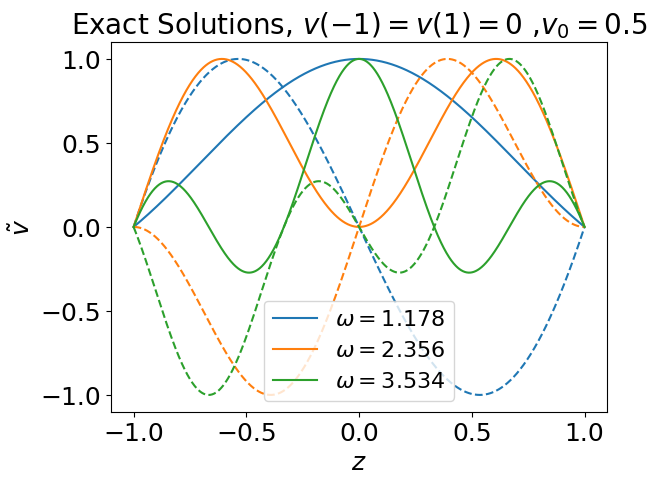
\includegraphics[width=\linewidth]{img/theoretical_analysis/exact_v0=0.5}
		\caption{Subsonic}
	\end{subfigure}%
	\begin{subfigure}{0.5\textwidth}
		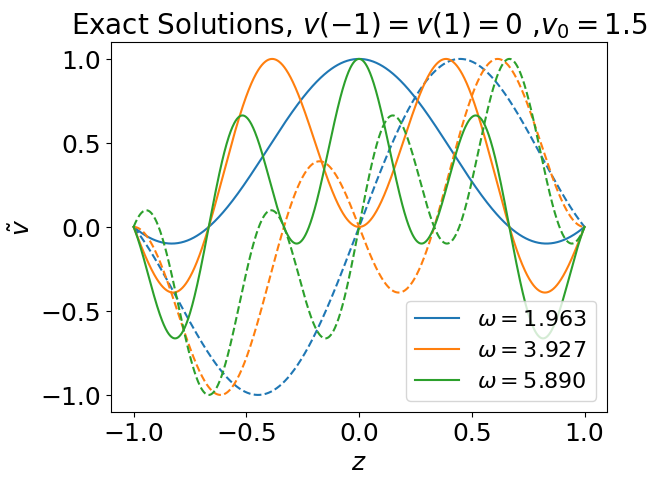
\includegraphics[width=\linewidth]{img/theoretical_analysis/exact_v0=1.5}
		\caption{Supersonic}
	\end{subfigure}
	\caption{The plots show the first three exact solutions to Eq.(\ref{eq:constant_v_problem_dirichlet}) for both subsonic and supersonic case. These solutions are stable.}
	\label{fig:exact_v}
\end{figure}


\section{Spectral Pollution and Spurious Modes}
In this section, we will discuss an important phenomenon we will observe throughout the numerical experiments. It is the phenomenon of spectral pollution.

Spectral pollution refers to the phenomenon which some eigenvalues are not converging to the correct value when the mesh density is increased. When solving eigenvalue problems using spectral methods with finite difference or finite element approximations, spectral pollution might occur. \cite{llobet_spectral_1990}

\subsection{Finite Difference Discretization of Operators}
In this section, we are going to investigate the spectral pollution phenomenon when solving Eq.(\ref{eq:constant_v_problem_dirichlet}) using spectral method.

The dispersion relation can be obtained by substituting $\tilde{v} = \exp(-i\omega t + kx)$ into Eq.(\ref{eq:constant_v_problem_dirichlet}),
\begin{equation} \label{dispersion_relation}
	\omega = k(v_0 \pm 1) 
\end{equation}

If we assume $v\sim \exp(ikx)$, and let $\beta\equiv kh/2$. Then in finite difference discretization scheme, the differential operators $\dv*[n]{z}$ are equivalent to the following factors \cite{llobet_spectral_1990},
\begin{align}
	&G_0 = 1 \nonumber \\
	&G_1 = [\exp(2i\beta)-\exp(-2i\beta)]/2h = (i/h)\sin(2\beta) 
	\label{G-operator}\\
	&G_2 = [\exp(2i\beta)-2-\exp(-2i\beta)]/h^2 = (2/h^2)(\cos(2\beta)-1) \nonumber 
\end{align}


\subsection{Analysis of Numerical Spectrum}
\subsubsection{Discretize on the Same Grid}
Using the G-operator, Eq.(\ref{G-operator}), the discretized equation of Eq.(\ref{eq:constant_v_problem_dirichlet}) is 
\begin{equation} \label{eq:discretized_eq_G}
    (\omega^2G_0 + \omega G_1 + G_2)\mathbf{\tilde{v}} = 0
\end{equation}
where $\mathbf{\tilde{v}}$ is the discretized vector of $\tilde{v}$.

Solving Eq.(\ref{eq:discretized_eq_G}), we obtain the numerical dispersion relation,
\begin{equation} \label{dispersion_relation_G}
	\omega = \frac{2\sin(\beta)}{h}\left(v_0 \pm \sqrt{1 - v_0^2\sin[2](\beta)}\right)
\end{equation}

Given $h$ (fixed the mesh resolution), we see that
\begin{itemize}
	\item $\omega$ is real for all $k$ if $v_0 < 1$.
	\item $\omega$ is complex for large $k$, more specifically $k>h/2\arcsin(1/v_0)$, if $v_0 > 1$.
	\item For small $k$, meaning $k\to 0$, Eq.(\ref{dispersion_relation_G}) is a good representation for the analytical dispersion relation, Eq.(\ref{dispersion_relation}). 
\end{itemize}
This explains why the spurious unstable modes occur when $v_0>1$.

\begin{figure}[H]
	\centering
	\begin{subfigure}[b]{0.5\linewidth}
		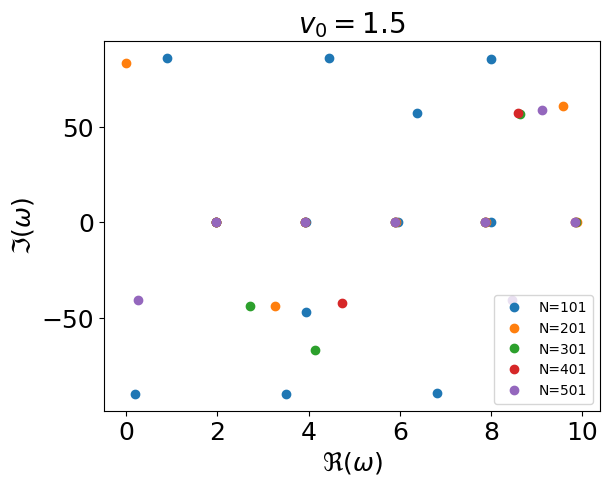
\includegraphics[width=\linewidth]{img/theoretical_analysis/eigvals_bad} 
		\caption{Bad eigenvalues}
	\end{subfigure}%
	\begin{subfigure}[b]{0.5\linewidth}
		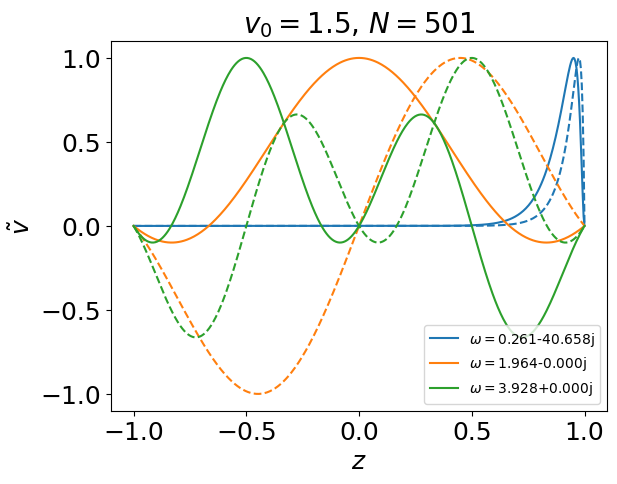
\includegraphics[width=\linewidth]{img/theoretical_analysis/eigvecs_bad} 
		\caption{Bad eigenfunctions}
	\end{subfigure}
	\caption{Spurious modes.}
	\label{fig:results_bad}
\end{figure}

One way to filter the spurious modes is to remove all modes with $k>h/2 \arcsin(1/v_0)$, see Fig.\ref{fig:results_filter_k}. However, this is not a good way to deal with general cases because it requires the solution to the discretized problem Eq.(\ref{eq:discretized_eq_G}). For general problem with non-constant velocity profile, it is hard to solve the discretized problem directly.

\begin{figure}[H]
	\centering
	\begin{subfigure}[b]{0.5\linewidth}
		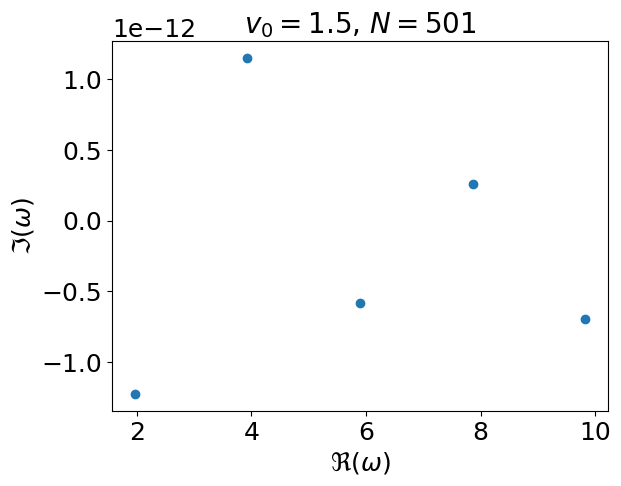
\includegraphics[width=\linewidth]{img/theoretical_analysis/eigvals_good} 
		\caption{Good eigenvalues}
	\end{subfigure}%
	\begin{subfigure}[b]{0.5\linewidth}
		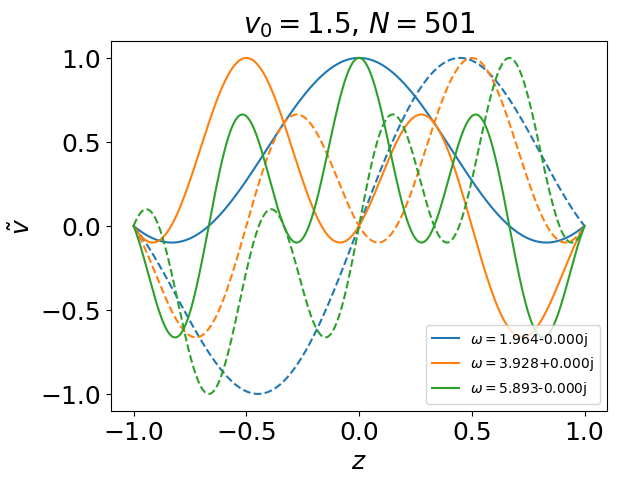
\includegraphics[width=\linewidth]{img/theoretical_analysis/eigvecs_good} 
		\caption{Good eigenfunctions}
	\end{subfigure}
	\caption{Filter out the spurious modes with $k>h/2\arcsin(1/v_0)$.}
	\label{fig:results_filter_k}
\end{figure}

A better way to filter the spurious modes is by doing a "convergence test". Since the frequency Eq.(\ref{dispersion_relation_G}) is changing with mesh resolution $h$. We can simply solve the discretized problem using spectral method under different mesh resolution. Then filter out the eigenmodes that are changing dramatically.

\section{Symmetry of Growth Rates in Accelerating and Decelerating Cases}
Notice that there exists a symmetry between the accelerating and decelerating velocity profiles. To be specific, these two profiles are symmetric about the axis $z=0$.
\[ v_a(-z) = v_d(z) \]
where the subscript $a$ stands for accelerating and $d$ stands for decelerating.

The symmetry between the two velocity profiles will lead us to the symmetry of growth rates between the accelerating case and decelerating case. 

\begin{proposition} \label{prop:symmetry_of_eigenvalue}
	If $\omega$ is an eigenvalue to the polynomial eigenvalue problem, Eq.\ref{eq:polynomial_eigenvalue_problem} width accelerating velocity profile $v_a(z)$, then its complex conjugate, $\overline{\omega}$, is an eigenvalue to the same equation with decelerating velocity profile, $v_d(z)$.
\end{proposition}
\begin{proof}
	Suppose $\omega=\omega_r + i\omega_i$ is an eigenvalue to Eq.\ref{eq:polynomial_eigenvalue_problem}. Substitute $\tilde{v}(z)$ by $\exp(ikz)$ and split the equation to real and imaginary part, we see that $\omega$ and $\omega_i$ must satisfy
	\begin{equation} \label{eq:eigenvalue_problem_real_part}
		\omega_r^2 - \omega_i^2 
		- 2\omega_r kv_0 - 2\omega_i\pdv{v_0}{z}
		+ \left[
		-k^2(1-v_0^2) 
		-\left(1-\frac{1}{v_0^2}\right)\left(\pdv{v_0}{z}\right)^2
		-\left(v_0+\frac{1}{v_0}\right)\pdv[2]{v_0}{z}
		\right]
		= 0
	\end{equation}
	\begin{equation} \label{eq:eigenvalue_problem_imag_part}
		2\omega_r\omega_i 
		- 2\omega_i kv_0 + 2\omega_r\pdv{v_0}{z} 
		- k\left(3v_0+\frac{1}{v_0}\right)\pdv{v_0}{z} 
		= 0
	\end{equation}
	Here the velocity profile $v_0$ can be accelerating, $v_a$, or decelerating, $v_d$.
	
	Since $v_d(z)=v_a(-z)$, so $\partial_zv_d=-\partial_zv_a$ and $\partial_z^2v_d=\partial_z^2v_a$. If the transformation $z\to -z$ is made, then Eq.\ref{eq:eigenvalue_problem_real_part} and Eq.\ref{eq:eigenvalue_problem_imag_part} become
	
	\[
		\omega_r^2 - \omega_i^2 
		- 2\omega_r kv_0' + 2\omega_i\pdv{v_0'}{z}
		+ \left[
		-k^2(1-v_0'^2) 
		-\left(1-\frac{1}{v_0'^2}\right)\left(\pdv{v_0'}{z}\right)^2
		-\left(v_0'+\frac{1}{v_0'}\right)\pdv[2]{v_0'}{z}
		\right]
		= 0
	\]
	\[
		2\omega_r\omega_i 
		- 2\omega_i kv_0' - 2\omega_r\pdv{v_0'}{z} 
		- k\left(3v_0'+\frac{1}{v_0'}\right)\pdv{v_0'}{z} 
		= 0
	\]
	where $v_0'(z) \equiv v_0(-z)$. We see that the imaginary part of the eigenvalue changes from $\omega_i$ to $-\omega_i$.
\end{proof}

\begin{remark}
	This proposition tells us that if the flow in magnetic nozzle is unstable in one case, then the flow will stable in the opposite case. More specifically, the perturbation is damped oscillation.
\end{remark}


\chapter{Numerical Experiments}
In this chapter, we will solve the eigenvalue problem, Eq.(\ref{eq:eigenvalue-problem}), with different discretizations. There will be three major categories of methods used. Finite difference (FD) method, finite element (FE) method and discrete variable representation (DVR) method.

The finite difference method will be used together with equally spaced nodes. The finite element method will be used with three different basis functions: tent function, B-spline and sine. Different basis function results in different discretization. Finally, sine DVR and sinc DVR will also be used to solve the eigenvalue problem.

The parameters of different discretizations are listed below
\begin{table} [H]
	\begin{tabular}{|c|c|c|c|c|c|c|}
		\hline
		& FD & FE\_TENT & FE\_BSPLINE & FE\_SINE & DVR\_SINE & DVR\_SINC \\
		\hline
		N & 201 &  &  &  &  &  \\
		\hline
		NUM\_BASIS &  & 15 & 21 & 50 & 31 & 39 \\
		\hline
	\end{tabular}
	\label{table:parameters}
\end{table}

\section{Constant Velocity}
Because the existence of exact solution to problems Eq.(\ref{eq:constant_v_problem_dirichlet}) and Eq.(\ref{eq:constant_v_problem_openright}). The case with constant velocity profile is used as a sanity check. It allows us to verify the correctness of each method's implementation. This also serves as a reference to the accuracy spectral methods can achieve.

From Fig.(\ref{fig:constant_v}), we see that the flow in magnetic nozzle with subsonic and supersonic velocity profile are both stable. The accuracy of spectral method is high, the imaginary part of eigenvalues are about $10^{-13}$.

\begin{figure}[H]
	\centering
	\begin{subfigure}{0.5\textwidth}
		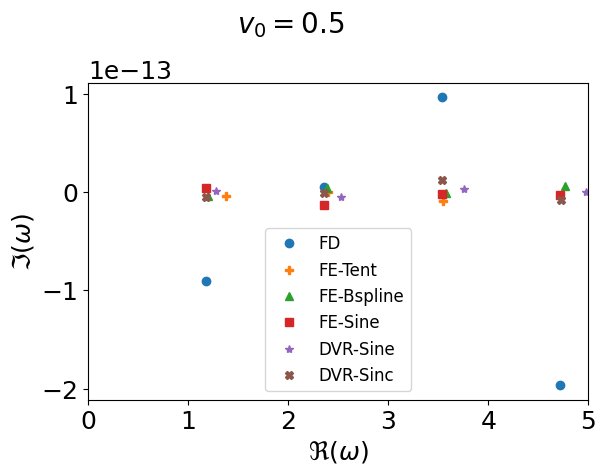
\includegraphics[width=\linewidth]{img/numerical_experiments/constant_v_v0=0.5}
		\caption{Subsonic}
	\end{subfigure}%
	\begin{subfigure}{0.5\textwidth}
		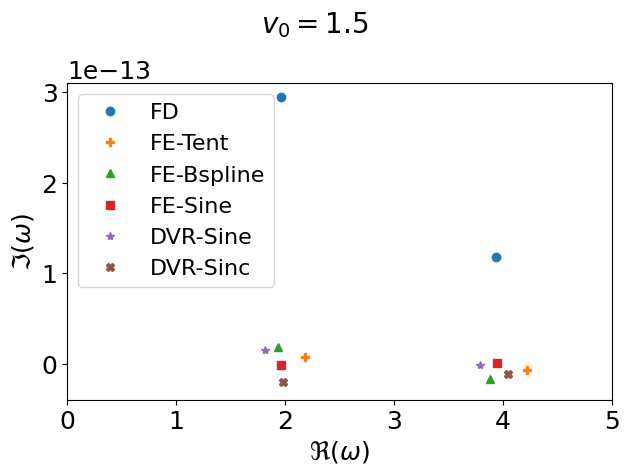
\includegraphics[width=\linewidth]{img/numerical_experiments/constant_v_v0=1.5}
		\caption{Supersonic}
	\end{subfigure}
	\caption{In subsonic case, all methods produces stable modes. In supersonic case, all modes are stable after filtering the spurious modes.}
	\label{fig:constant_v}
\end{figure}


\section{Subsonic Case}
\subsection{Fixed Ends}
With Dirichlet boundary condition, $\tilde{v}(\pm 1) =0$. The flow in magnetic nozzle with subsonic velocity profile is stable. Fig.\ref{fig:subsonic_v} shows the first few eigenvalues obtained by different discretizations, they all produced similar results.
\begin{figure} [H]
	\centering
	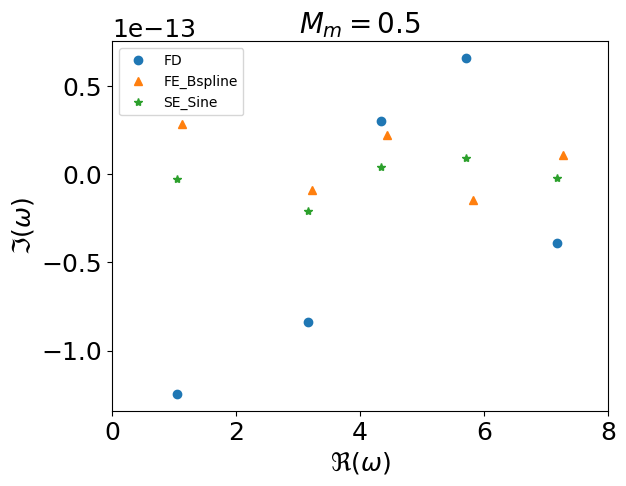
\includegraphics[width=0.7\linewidth]{img/numerical_experiments/subsonic_v}
	\caption{The flow is stable.}
	\label{fig:subsonic_v}
\end{figure}

\subsection{Open Right End}


\section{Supersonic Case}
\subsection{Fixed Ends}
When the velocity profile is supersonic, spurious modes appeared as predicted in Chap.\ref{chap:theoretical_analysis}. Using the convergence test, we successfully eliminates all spurious modes. Fig.(\ref{fig:supersonic_v}) shows the first few filtered eigenvalues. As we can see the flow is stable.
\begin{figure} [H]
	\centering
	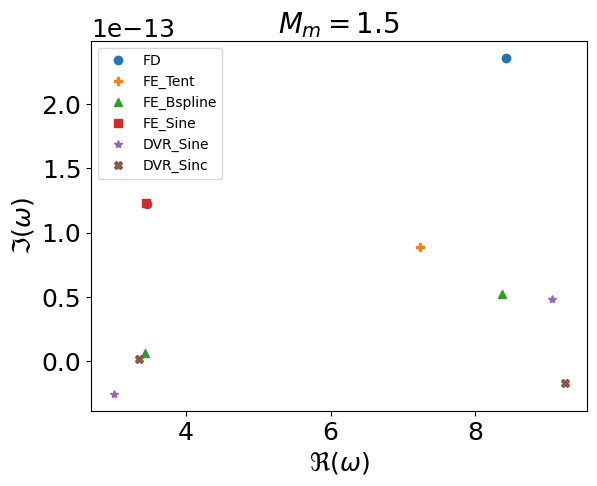
\includegraphics[width=0.7\linewidth]{img/numerical_experiments/supersonic_v}
	\caption{First few filtered eigenvalues are shown. The spurious modes are filtered by convergence test.}
	\label{fig:supersonic_v}
\end{figure}

\subsection{Open Right Ends}


\section{Accelerating Case}
In this case, the flow starts from subsonic speed and accelerates to supersonic case, the velocity is exactly at sonic point $M_m=1$ at the center of the magnetic nozzle as shown in Fig.(\ref{fig:velocity_profiles})
\subsection{Fixed Ends}
With Dirichlet boundary condition, spectral method with different discretizations gave negative eigenvalues. This indicates that the perturbation $\tilde{v}$ is damped oscillation, its amplitude will be decrease to zero exponentially in time, $\tilde{v} \sim \exp(\Im(\omega)t)$. Hence, the flow in magnetic nozzle is stable.
\begin{figure} [H]
	\centering
	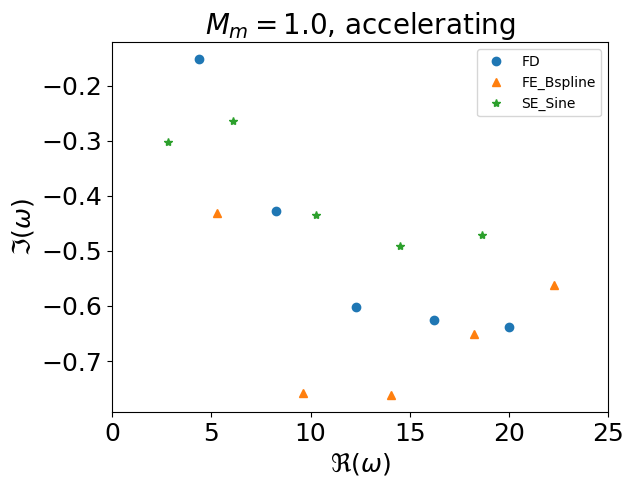
\includegraphics[width=0.7\linewidth]{img/numerical_experiments/accelerating_v}
	\caption{The filtered eigenvalues are negative. This indicates that the perturbation $\tilde{v}$ is a damped oscillation, their amplitude will decrease to zero as time elapse.}
	\label{fig:accelerating_v}
\end{figure}

\subsection{Open Right Ends}


\section{Decelerating Case}
\subsection{Fixed Ends}
Let $v_a(z)$ denotes the accelerating velocity profile, and $v_d(z)$ the decelerating velocity profile. Then we know $v_a(-z) = v_d(z)$.

The eigenvalue problem with accelerating profile is given by
\[
	\hspace{-0.5in}
	\omega^2 \tilde{v} 
	+ 2i\omega\left(v_a\pdv{}{z} + \pdv{v_a}{z}\right) \tilde{v} 
	+ \left[ (1-v_a^2)\pdv[2]{}{z} 
	-\left(3v_a + \frac{1}{v_a}\right)\pdv{v_a}{z}\pdv{}{z} 
	- \left(1-\frac{1}{v_a^2}\right)\left(\pdv{v_a}{z}\right)^2 
	- \left(v_a+\frac{1}{v_a}\right)\pdv[2]{v_a}{z} \right]\tilde{v}
	= 0
\]
Let $z\mapsto -z$, the eigenvalue problem becomes
\[
	\hspace{-1.5in}
	\omega^2 \tilde{v} 
	+ 2i\omega\left(v_d\pdv{}{(-z)} + \pdv{v_d}{(-z)}\right) \tilde{v} 
	+ \left[ (1-v_d^2)\pdv[2]{}{(-z)} 
	-\left(3v_d + \frac{1}{v_d}\right)\pdv{v_d}{(-z)}\pdv{}{(-z)} 
	- \left(1-\frac{1}{v_d^2}\right)\left(\pdv{v_d}{(-z)}\right)^2 
	- \left(v_d+\frac{1}{v_d}\right)\pdv[2]{v_d}{(-z)} \right]\tilde{v}
	= 0
\]
Hence, we have
\[
\hspace{-0.5in}
\omega^2 \tilde{v} 
- 2i\omega\left(v_d\pdv{}{z} + \pdv{v_d}{z}\right) \tilde{v} 
+ \left[ (1-v_d^2)\pdv[2]{}{z} 
-\left(3v_d + \frac{1}{v_d}\right)\pdv{v_d}{z}\pdv{}{z} 
- \left(1-\frac{1}{v_d^2}\right)\left(\pdv{v_d}{z}\right)^2 
- \left(v_d+\frac{1}{v_d}\right)\pdv[2]{v_d}{z} \right]\tilde{v}
= 0
\]

We see that the flow with decelerating profile is a different physical process than the that with accelerating profile.

\begin{figure} [H]
	\centering
	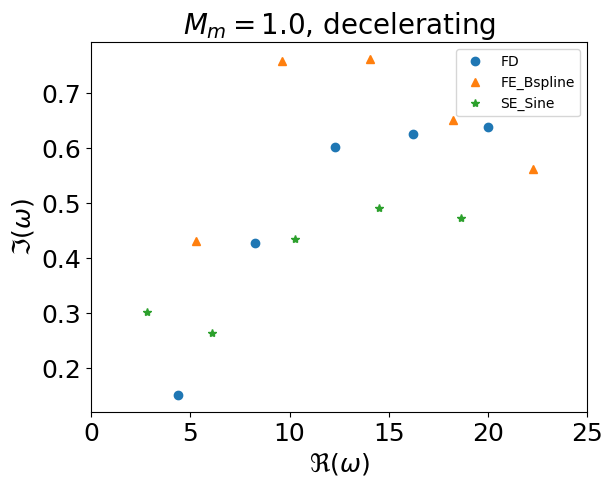
\includegraphics[width=0.7\linewidth]{img/numerical_experiments/decelerating_v}
	\caption{Unstable}
	\label{fig:decelerating_v}
\end{figure}

\subsection{Open Right Ends}

\chapter{conclusion}

\bibliographystyle{plain}
\bibliography{references} 

\end{document}
